% Conditional flow matching.  Build: latexmk -pdf flow.tex
\documentclass[border=8pt]{standalone}
\usepackage{amsmath}
% Shared TikZ palette + node styles for the ML-RT2 architecture diagrams.
% Colours match the ML-RT comparison-paper figures so the three papers look consistent:
%   pink   = data / vectors (inputs, outputs, latent representations)
%   blue   = learned networks / operators (MLPs, encoders, decoders, ...)
%   orange = special operations / physics (spectral transforms, RT residual, ...)
%   green  = loss / training terms
\usepackage{tikz}
\usetikzlibrary{arrows.meta,positioning,fit,backgrounds,calc}

\definecolor{dataFill}{HTML}{F2E6FF}\definecolor{dataDraw}{HTML}{6600CC}
\definecolor{netFill}{HTML}{B5E8E8}\definecolor{netDraw}{HTML}{086565}
\definecolor{opFill}{HTML}{FFE0C2}\definecolor{opDraw}{HTML}{AB4F03}
\definecolor{lossFill}{HTML}{C8F4C1}\definecolor{lossDraw}{HTML}{0C5600}

\tikzset{
  font=\small,
  box/.style  ={draw, rounded corners, align=center, inner sep=4pt, minimum height=9mm, line width=0.3mm},
  data/.style ={box, fill=dataFill, draw=dataDraw},
  net/.style  ={box, fill=netFill,  draw=netDraw},
  op/.style   ={box, fill=opFill,   draw=opDraw},
  loss/.style ={box, fill=lossFill, draw=lossDraw},
  sum/.style  ={draw=netDraw, circle, inner sep=1.3pt, fill=white, line width=0.3mm},
  arr/.style  ={-{Stealth[length=2.4mm]}, thick},
  darr/.style ={-{Stealth[length=2.4mm]}, thick, dashed},
  note/.style ={align=center, font=\scriptsize, text=black!65},
}

\begin{document}
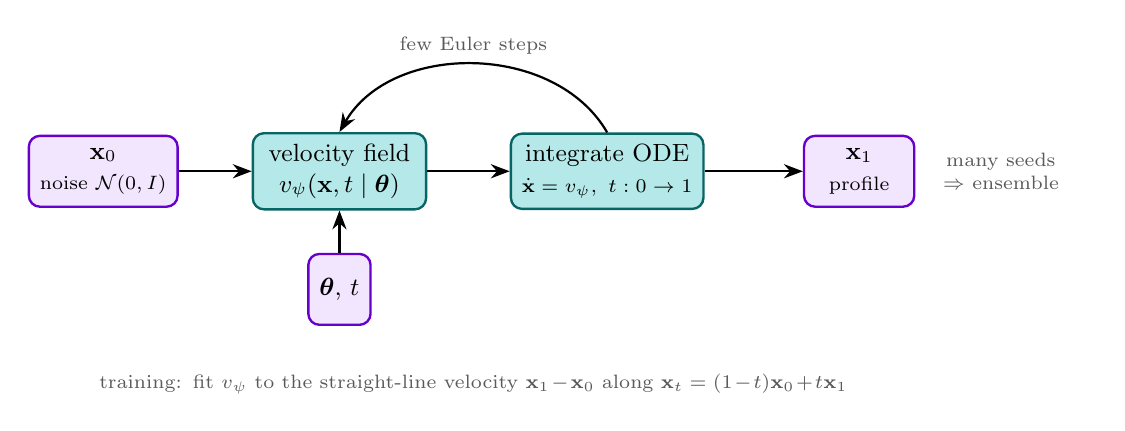
\begin{tikzpicture}
  \node[data] (x0)                       at (0,0)    {$\mathbf{x}_0$\\{\scriptsize noise $\mathcal{N}(0,I)$}};
  \node[net,  minimum width=22mm] (v)    at (3.0,0)  {velocity field\\$v_\psi(\mathbf{x},t\mid\boldsymbol{\theta})$};
  \node[net,  minimum width=20mm] (int)  at (6.4,0)  {integrate ODE\\{\scriptsize $\dot{\mathbf{x}}=v_\psi,\ t:0\to1$}};
  \node[data, minimum width=14mm] (x1)   at (9.6,0)  {$\mathbf{x}_1$\\{\scriptsize profile}};
  \draw[arr] (x0)--(v); \draw[arr] (v)--(int); \draw[arr] (int)--(x1);

  \node[data] (th) at (3.0,-1.5) {$\boldsymbol{\theta}$, $t$};
  \draw[arr] (th) -- (v);
  \draw[arr] (int.north) to[out=120,in=60] node[above, note] {few Euler steps} (v.north);

  \node[note, text width=22mm] at (11.4,0) {many seeds\\$\Rightarrow$ ensemble};
  \node[note, text width=95mm] at (4.7,-2.7)
    {training: fit $v_\psi$ to the straight-line velocity $\mathbf{x}_1-\mathbf{x}_0$ along
     $\mathbf{x}_t=(1-t)\mathbf{x}_0+t\mathbf{x}_1$};
\end{tikzpicture}
\end{document}
